% Page style for this chapter
	\pagestyle{fancy}
	\lhead{{\sffamily \MakeUppercase{8. Time-Dependent Effects}}}
	\chead{}
	\rhead{{\sffamily \MakeUppercase\rightmark}}
	\lfoot{}
	\cfoot{{\sffamily \thepage}}
	\rfoot{}

\setstretchnormal

\chapter{Incorporating Time-Dependent Effects into Models of the Cochlea}
\label{sect:time_dependency}

% Textbox
\begin{center}
	\begin{tcolorbox}[title=\boxtitle]
		\begin{itemize}[leftmargin=*,labelindent=2ex,labelsep=1.5ex,itemsep=0pt,parsep=0pt]
			\item Are time-dependent effects important in volume conduction?
			\item How could these effects be modelled?
			\item What are the implications of these effects?
		\end{itemize}
	\end{tcolorbox}
\end{center}

%% ====================================================== Time-Dependent Effects

\section{Introduction}

% General quasi-static stuff
All of the volume conduction models (VCMs) discussed in
\S\ref{sect:volume_conduction_models} are different in terms of appearance and
methodology, yet they share the key assumption of \emph{quasi-stationarity}.
Quasi-static models have in fact been used in most electrophysiological
studies~\cite{plonsey1967}, enabling the use of relatively simple stationary
(i.e. time-independent) formulations. If valid, this assumption implies that all
field components in the system will be synchronous and greatly reduces
computational requirements.

However, the quasi-static assumption should only be invoked if a number of
conditions are met. According to Plonsey~\cite{plonsey1967}, these are:
\begin{itemize}[after=\vspace{1.5\medskipamount}]
    \item Propagation can be neglected.
    \item Capacitive effects can be neglected.
    \item Inductive effects can be neglected.
    \item The system is bounded by a region of zero conductivity.
\end{itemize}

The weakest of the four conditions is that capacitive effects can be neglected
or, equivalently, that the conductivity of the medium dominates its
behaviour~\cite{plonsey1967}. This is only true if:
\begin{equation}
	\frac{\omega \epsilon(\omega)}{\sigma(\omega)} \ll 1
	\label{eqn:quasi-static_1}
\end{equation}
where $ \omega = 2 \pi f $ is the angular frequency of the stimulus, $ \epsilon
$ is the absolute permittivity of the medium, and $ \sigma $ is the conductivity
of the medium~\cite{plonsey1967}. Here, the ``$ \ll $'' comparator is
interpreted as requiring a reduction of at least one order of magnitude. It is
important to note that the conductivity and permittivity of materials is a
function of frequency, especially for biological
tissues~\cite{schwan1957capacitive,schwan1957conductivity,gabriel1996b}.

Equation~\ref{eqn:quasi-static_1} can also be written as:
\begin{equation}
	\frac{\omega \epsilon_0 \epsilon_r(\omega)}{\sigma(\omega)} \ll 1
	\label{eqn:quasi-static_2}
\end{equation}
where $ \epsilon_0 $ is the permittivity of free space, and $ \epsilon_r $ is
the relative permittivity of the medium. Equation~\ref{eqn:quasi-static_2} will
henceforth be referred to as the quasi-static criterion (QSC).

% Evidence used for pure resistivity in the cochlea
Existing models of the implanted cochlea have all assumed that the cochlear
tissues are purely resistive in order to satisfy the QSC. There are a few
reasons for this, beginning with the fact that the fundamental frequency of the
input pulses used in cochlear implant (CI) systems is relatively low, typically
around 10--20~kHz~\cite{vanpoucke2004identification}. At these frequencies,
conductive effects are expected to dominate~\cite{grimnes2000}. Early
experimental work seemed to support this: von \bekesy{} reported observing no
capacitive component when measuring impedances with a 1000~Hz pure tone
stimulus~\cite{vonbekesy1951}, and Spelman demonstrated minimal phase lag in his
experiments with broadband (8--12,500 Hz) white noise current waveforms in the
scala tympani of the guinea pig~\cite{spelman1982}. Spelman concluded that the
system is primarily resistive in nature, and his paper is often cited as
justification for using purely resistive material models (see, for example,
Girzon~\cite{girzon1987}, Finley~\cite{finley1990}, Frijns~\cite{frijns1995},
and Hanekom~\cite{hanekom2001}).

% Biology is not simply resistive
However, it is well known that biological tissues are not purely resistive. The
presence of proteins and amino acids in the fluids of the inner ear (cf.
Table~\ref{table:fluid_composition}) endows them with a small capacitive
component~\cite{grimnes2000}. The other two dominant tissues in the inner ear,
bone and nerve, which have been found to be major determinants of the current
pathways, both have well documented dielectric
responses~\cite{williams1996,gabriel1996b,brown2001}. Blood is also capacitive
due to the cell walls of erythrocytes and proteins in the
plasma~\cite{grimnes2000}.

While the frequency-dependent conductivities and permittivities of more general
bodily tissues have been measured, there is no permittivity data for
cochlear-specific tissues, and measurements of the conductivity values have only
been performed in a narrow range of frequencies. This has been the biggest
barrier to performing time-dependent cochlear studies \insilico. Data that is
available for general tissues can provide some guidelines though. The IT'IS
Foundation database~\cite{hasgall2015} is the most comprehensive source of
dielectric tissue properties at the time of writing. This database consolidates
the data of Geddes and Baker~\cite{geddes1967}, Gabriel
\etal{}~\cite{gabriel1996a,gabriel1996b,gabriel1996c}, and many others into an
interactive online compendium, building upon the earlier work of
Andreuccetti~\cite{andreuccetti2000}.

Table~\ref{table:quasi-static_criterion} shows the QSC calculated for some of
the tissues in the database that might be applied to models of the cochlea. At a
frequency of 10~kHz, the QSC values for most tissues are less than 0.015, which
suggests that the quasi-static assumption is reasonable. However, the QSC for
nerve tissue is not substantially less than unity. The criterion is directly
proportional to frequency, and at 10~MHz the values for most tissues are much
higher. At this higher frequency, only cerebrospinal fluid (CSF) satisfies the
QSC.

\begin{table}
	\centering
	\sffamily
	\small
	\caption[Quasi-static criterion values at 10 kHz and 10 MHz]{Quasi-static
	criterion values for some comparable tissues at both 10 kHz and 10 MHz. The
	frequency-dependent tissue properties were sourced from the IT'IS Foundation
	database~\cite{hasgall2015}. For most tissues, the criterion is not
	substantially less than one at the higher frequency as per
	Equation~\ref{eqn:quasi-static_2}.}
	\label{table:quasi-static_criterion}
	
	\begin{tabularx}{0.5\textwidth}{X c c}
		\toprule
		\textbf{Tissue}	& \multicolumn{2}{c}{\textbf{Quasi-static criterion}} \\
						& \textbf{~~10 kHz~~}	& \textbf{~~10 MHz~~} \\
		\midrule
		\csvreader[late after line=\\]%
			{Simulations/TimeDep/quasi-static_criterion.csv}%
			{1=\tissue,2=\fund,3=\harm}%
 			{\tissue & \fund & \harm}%
		\bottomrule
	\end{tabularx}
	
\end{table}

% Square pulse stuff
There are two main implications of these data. The first is that higher
frequency components of the stimulus may play a non-trivial role in determining
the field quantities. Higher frequency components are seen in clinical practice
because CIs deliver charge into the cochlea using square, biphasic,
constant-current pulses (see Figure~\ref{fig:biphasic_pulse}). The biphasic
nature of the stimulus means it is an alternating current (AC) signal, and its
square shape means that it is not a pure tone but a combination of the
fundamental frequency and higher frequency harmonics, as revealed when
considering its Fourier transformation. These high frequency components are
important in describing the relatively sharp rising and falling
edges~\cite{kreyszig1988,tognola2007}. Therefore, the stimulus should not be
modelled as a simple direct current (DC) signal.

% Nerve stuff
The second implication draws from the relatively high QSC value for nerve
regardless of frequency as shown in Figure~\ref{fig:nerve_qsc}, which indicates
that quasi-stationary results are not valid in those regions. This is worrisome
for VCMs with coupled neural models because they assume that the extracellular
potential in the nerve tissue is time-invariant~\cite{mcneal1976}; the high QSC
value suggests that the electric field does change over time. Since neural
excitation is a function of voltage differences in the nerve tissue,
fluctuations in the extracellular potential may have a large impact on
predictions of neural excitation, depending on the sensitivity of the model.
Despite concerns from early studies that purely resistive models of the cochlea
should only be considered as a first
approximation~\cite{finley1990,frijns1995,hanekom2001}, no subsequent studies
have properly considered the validity of this assumption.

\begin{figure}
	\centering
	\includegraphics[height=7cm]{Simulations/TimeDep/nerve_qsc}
	\caption[Quasi-static criterion for nerve tissue]{Quasi-static criterion for
	nerve tissue, up to 1~GHz. The values vary with frequency and are generally not
	significantly less than unity (dashed line).}
	\label{fig:nerve_qsc}
\end{figure} 

% For discussion?

% However, Spelman was only shown to be true for measurements within the scala
% tympani. Assumption based on incorrect interpretation of data by Spelman. Only
% true for measurements within the scala tympani. What about at other points?

% The field quantities simply scale proportionally with the amplitude of the input
% current under a purely resistive formulation~\cite{plonsey1967}

% From streamlines, see that current follows a path, hits ST first, so no freq
% dependent build up of charge? (Theory only, could be incorrect to interpret in
% terms of spatial movement.)
% 
% Strelioff (Intro, paragraph 1)---neural excitation effects requires estimation
% of both spatial and temporal distribution of electric currents in the nerve.

% Platinum resembles a \emph{perfectly polarisable electrode}---no charge actually
% crosses the interface, the current is a displacement current. This changes the
% concentration of ions at the surface, resulting in a concentration overpotential
% (only for measuring?) that results in a strong capacitive
% effect~\cite{webster1998}.

As such, the aim of this chapter is to address this long-standing concern by
exploring the feasibility of performing time-dependent simulations of the
implanted cochlea, documenting observed differences between otherwise equivalent
quasi-static and time-dependent models, and extrapolating how these differences
might affect the predictions in both this and other modelling efforts. Some
early work on this topic, based on an updated iteration of the proof of concept
model, was published at the IEEE Conference on Neural Engineering
2015~\cite{inguva2015ner}. A refined methodology has been applied to the guinea
pig model for the present study.

\section{Method}

In order to model time-dependent effects, the stimulating pulse was converted
from the time domain into its equivalent frequency-domain representation via
Fourier analysis (as suggested by Plonsey~\cite{plonsey1967}) before the
numerical solution. The model was then set up and solved across the range of
frequencies in COMSOL, after which the field results were reconstructed in
MATLAB to produce a time-domain signal representing the dynamics of the field
interactions. This procedure is illustrated schematically in
Figure~\ref{fig:td_method_summary}.

\begin{figure}
	\centering
	\includegraphics[width=\textwidth]{Simulations/TimeDep/method_summary}
	\caption[Schematic of the solution process for time-dependent
	simulations]{Schematic of the solution process for time-dependent simulations.
	The time-domain stimulus was decomposed into its spectral components via a
	Fourier transformation. The response at each frequency was analysed in COMSOL,
	and the outputs later recombined to obtain the corresponding transient
	response. (Copyright \textcopyright{} 2015, IEEE.)}
	\label{fig:td_method_summary}
\end{figure}

\subsection{Fourier Expansion of the Stimulating Pulse}

Consider a periodic time-domain signal with period $ 2L $. This function, $ F(t)
$, can be decomposed into its Fourier components, given by:
\begin{equation}
	F(t) = \sum_{n=0}^\infty a_n \cos n \omega t + b_n \sin n \omega t
	\label{eqn:fourier_general}
\end{equation}
\renewcommand{\arraystretch}{0.9}
\begin{equation}
	\begin{pmatrix} a_n \\ b_n \end{pmatrix} = \frac{1}{N_n} \int_0^{2L} F(t)
	\begin{pmatrix} \cos n \omega t \\ \sin n \omega t \end{pmatrix} \, dt
	\label{eqn:fourier_coefficients_general}
\end{equation}

\renewcommand{\arraystretch}{1.3}

where $ n $ is a non-negative integer, $ \omega $ is the \emph{fundamental
frequency} in radians per second, given by $ \omega $ = 2$ \pi $/period = $ \pi
/ L $, and the normalisation factor is $ N_n $ = $ L(1+ \delta_{n0}) $, with $
\delta $ being the Kronecker delta function~\cite{kreyszig1988}.

If $ F(t) $ is an odd function, $ a_n $ = 0, so the Fourier series reduces to a
pure sine expansion and
Equations~\ref{eqn:fourier_general}--\ref{eqn:fourier_coefficients_general}
become:\vspace{1ex}
\begin{equation}
	F(t) = \sum_{n=1}^\infty b_n \sin n \omega t
	\label{eqn:fourier_odd}
\end{equation}
\begin{equation}
	b_n = \frac{1}{N_n} \int_0^{2L} F(t) \sin n \omega t \, dt
	\label{eqn:fourier_coefficients_odd}
\end{equation}

Equations~\ref{eqn:fourier_odd}--\ref{eqn:fourier_coefficients_odd} can be used
to simplify the simulation. Consider a biphasic pulse train as illustrated
schematically in Figure~\ref{fig:biphasic_pulse}. By shifting the phase of the
signal such that the midpoint of an inter-frame gap (IFG) occurs at time $ t=0
$, $ F(t) $ becomes an odd function. Therefore, the original time-domain signal
can be approximated by using sine terms only, halving the number of simulations
required to compute the solution.

The base case stimulus waveform for the following time-dependent simulations is
shown in Figure~\ref{fig:base_stimulus}. It has a period of 100~$ \upmu $s,
giving it a fundamental frequency of 10~kHz. A 25~$ \upmu $s pulse width (PW) is
used for both cathodic and anodic phases, separated by an inter-phase gap (IPG)
of 10~$ \upmu $s. The amplitude of the pulse is 1~mA. The waveform was
programmed into COMSOL parametrically so that the input stimulus could be
modified easily. The relevant settings are shown in
Figure~\ref{fig:COMSOL_waveform}.

\begin{figure}
	\centering
	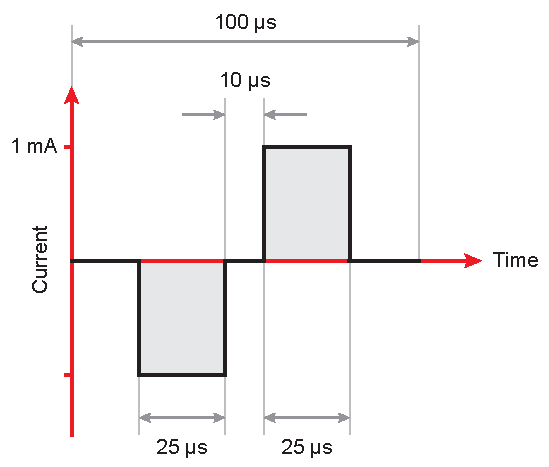
\includegraphics[height=7.5cm]{Simulations/TimeDep/base_stimulus}
	\caption[The base case stimulus waveform]{The base case stimulus waveform used
	for the time-dependent simulations. The inter-frame gap is driven by the other
	intervals, with onset of the cathodic phase occurring at the midpoint of the
	inter-frame gap to ensure that the function is odd.}
	\label{fig:base_stimulus}
\end{figure}

\begin{figure}[p]
    \centering
    
    \begin{subfigure}[t]{\textwidth}
        \centering
        \includegraphics[width=7.5cm]{Simulations/TimeDep/COMSOL_params_crop}
        \caption{}
        \label{fig:COMSOL_params}
    \end{subfigure}\\%
    \vspace{1em}%
	\begin{subfigure}[t]{0.49\textwidth}
        \centering
        \includegraphics[width=7.5cm]{Simulations/TimeDep/COMSOL_analytic_crop}
        \caption{}
        \label{fig:COMSOL_analytic}
    \end{subfigure}%
	\hfill%
    \begin{subfigure}[t]{0.49\textwidth}
        \centering
        \includegraphics[width=7.5cm]{Simulations/TimeDep/COMSOL_freqSol_crop}
        \caption{}
        \label{fig:COMSOL_freqSol}
    \end{subfigure}
    
	\caption[Parametric implementation of the stimulus waveform]{Parametric
	implementation of the stimulus waveform in COMSOL. (a) The parameters defining
	the stimulus waveform; (b) the expression for the Fourier transform; (c) the
	frequency sweep used in the solution. Temporal and angular frequencies were
	related by defining a model variable.}
	\label{fig:COMSOL_waveform}
\end{figure}

Although Equations~\ref{eqn:fourier_general} and \ref{eqn:fourier_odd} stipulate
the sum of an infinite number of harmonic terms, the marginal impact of an
additional frequency component progressively diminishes. The series does
converge, with similar previous studies requiring in the order of 500--5000
harmonics to achieve reasonably-shaped
waveforms~\cite{butson2005,bossetti2008,inguva2015ner}. However, the overshoot
that appears at the discontinuities of $ F(t) $ is a result of the non-uniform
convergence at those points and cannot be entirely
removed~\cite{kreyszig1988}---this is known as the \emph{Gibbs phenomenon}. In
this study, a total of 5000 harmonics was solved to test for convergence. The
corresponding frequency range extended up to 50~MHz.

An analytic function describing the stimulus waveform was then applied as the
input current at electrode E4. Since the simulations were performed using the
guinea pig model, the overall amplitude was set to 1~mA. As the frequency sweep
stepped through each harmonic in the specified range, the system was solved with
the weighted input current specific to that harmonic frequency. The model was
grounded at the temporal bone surface because the voltage offset boundary
condition was based on a full 1~mA stimulus and thus inappropriate for lower
magnitude current components.

Note that the capacitance at the electrode-tissue interface was not incorporated
here. This is because the study was more interested in quantities in the tissue,
and the current delivered to the tissues would not depend on the polarisation
voltage at the electrode surface due to the constant current nature of the
stimulus~\cite{grimnes2000}. This does however have a bearing on comparisons
with \invivo{} measurements.

\subsection{Assignment of Frequency-Dependent Material Properties}

The model was formulated in the frequency domain, so it was necessary to assign
frequency-dependent tissue properties. The main difficulty here was the lack of
suitable, cochlear-specific tissue data. As a first venture into this area
though, a rudimentary methodology would suffice. The model was previously found
to be most sensitive to the resistivities of bone, perilymph, and nerve in the
stationary simulations (see Chapter~\ref{sect:validation}). These tissues also
made up a majority of the cochlear volume, so it was plausible to assume that
these were the key drivers in a time-dependent formulation. The available data
for each of these was considered carefully.

For bone tissue, the IT'IS database listed separate entries for cortical and
cancellous bone. In light of the morphological differences in the cochlear bone,
the conductivity and permittivity of cortical bone were assigned to the denser
otic capsule, while the properties of cancellous bone were assigned to the
softer modiolar bone. Given that the petrous part of the temporal bone is known
to be extremely hard~\cite{bast1949,cooper1975}, the surrounding bone was also
modelled as cortical bone. In a similar fashion, the model domains representing
the peripheral processes, spiral ganglion, and auditory nerve trunk were
modelled using the listed data for nerve tissue.

The closest candidate for perilymph was CSF. Table~\ref{table:fluid_composition}
documents the compositions of the two fluids and reveals that they are
remarkably similar, as pointed out by Martini~\cite{martini2006}. However, there
are substantial differences in their protein content, which is known to have an
impact on electric properties~\cite{grimnes2000}. Due to this uncertainty and
the evidence of minimal phase lag in the scala tympani~\cite{spelman1982}, it
was decided to retain the assumption of pure resistivity for perilymph, as well
as endolymph.
% The QSC for CSF was relatively small, even at higher frequencies (reaching
% 0.13729 at 50~MHz). Worth using as lower bound?
The actual CSF in the model was of course assigned with the available
material properties.

The other two tissues that were assigned frequency-dependent properties were
blood and the spiral ligament. The latter used the value listed for
tendon/ligament. Neither are expected to have a significant impact on the
result given their comparatively low QSC values, but these values were not low
enough to warrant complete omission.

For all of the tissues discussed above, the values for both conductivity and
permittivity were pulled from the IT'IS database in the frequency range of
1~kHz to 100~MHz. This provided some leeway on either side of the frequency
sweep range used in the model solution. Values between the data points were
interpolated in COMSOL using cubic splines, an example of which is shown in
Figure~\ref{fig:COMSOL_nerve_cond_interp}. All other cochlear tissues were
modelled as purely resistive as per previous solutions since no better data were
available.

\begin{figure}
	\centering
	\includegraphics[height=6.2cm]{Simulations/TimeDep/nerve_cond_interp}
	\caption[Interpolation of nerve conductivity in COMSOL]{Interpolation of nerve
	conductivity in COMSOL. Data was sourced from the IT'IS
	Foundation~\cite{hasgall2015}.}
	\label{fig:COMSOL_nerve_cond_interp}
\end{figure}

\subsection{Reconstruction of the Time-Domain Signal}

Frequency-domain simulation outputs are represented in COMSOL as complex
quantities. The quantity values for a single frequency component can be written
in modulus-argument form, representing the amplitude and phase of the quantity
respectively, as:
\begin{equation}
	Z = A \, \mathrm{cis} \, \phi
	\label{eqn:complex_output}
\end{equation}
where $ Z $ is the output quantity, $ A $ is the amplitude of the signal, cis
is the complex exponential function, and $ \phi $ is the phase. Reconstructing
the corresponding time domain signal is simply a matter of summing each frequency
component while accounting for the phase shift. Since the input signal was
formulated as per Equation~\ref{eqn:fourier_odd}, only sine terms were required
for the reconstruction, that is:
\begin{equation}
	G(t) = \sum_{n=1}^N A_n \sin(n \omega t + \phi_n)
	\label{eqn:fourier_recon}
\end{equation}
where $ G(t) $ is the reconstructed signal and $ N $ is the total number of
harmonics used. The reconstructions for this study were scripted in MATLAB.

\subsection{Resistive Formulation}

In order to provide a more direct comparison with these time-dependent results,
a purely resistive counterpart was required. The stationary models from earlier
chapters were not used for this because the data sources for some of the tissue
properties were different. Instead, a new stationary model was created where
those tissues that could be modelled with frequency-dependent values (namely
bone, nerve, CSF, blood, and spiral ligament) were assigned their corresponding
conductivity values at the fundamental frequency. Relative permittivities for
all tissues were set to unity.

Since the calculated field quantities are synchronous with the rise and fall of
the input current in a purely resistive formulation~\cite{plonsey1967}, the temporal
waveform was identical in shape to that of the stimulus. The amplitudes were set
to the corresponding solution values.

\section{Results}

\subsection{Solution Times}

Since the simulations were solved as a string of stationary analyses (one for
each harmonic in the sweep), it was not surprising to find that solution times
scaled in a very linear fashion. Representative solution times are listed in
Table~\ref{table:td_solution_times}. The stationary study with linear
discretisation consisted of 793,311 degrees of freedom (DOFs) and took about 1.5
minutes to compute using the PARDISO solver. For comparison, a simulation with
100 harmonics took just over 2.5 hours to complete, while 5000 harmonics took
about 5 days and 8 hours.

\begin{table}
	\centering
	\sffamily
	\small
	
	\caption[Solution times for the time-dependent model]{Solution times for the
	time-dependent model. Note that the mesh was linearly discretised.}
	\label{table:td_solution_times}
	
    \begin{tabular}{l r}
	\toprule
	\textbf{Number of harmonics}	& \textbf{~~Solution time} \\
	\midrule
	
	1 (stationary)	& 1 min 26 secs \\
	100				& 2 hrs 33 mins \\
	5000			& 5 days 8 hrs \\
	\bottomrule
	\end{tabular}
\end{table}

% Linear discretisation

% Number of degrees of freedom solved for: 793311.
% Solution time (Solver 1 {sol1}): 86 s. (1 minute, 26 seconds)

% For 100, 500, and 5000 harmonics, official times were: 2h 32m 32s; 12h 28m
% 48s; 5d 7h 54m 42s, respectively

\subsection{Convergence of the Stimulus Waveform}

Since the overall solution time increased with the number of harmonics used, it
was desirable to find a balance between the two that yielded reasonable results.
Too few harmonics would lead to a poorly shaped stimulus (and consequently,
poorly shaped outputs); too many would be an inefficient use of computational
resources with negligible marginal benefit.

\subsubsection{Comparison of Square and Ramped Stimuli}

The first test involved reconstructing square biphasic stimuli to varying
degrees of accuracy to determine how this affects the shape of the waveform. For
the square-shaped biphasic stimulus shown in Figure~\ref{fig:base_stimulus}, the
accuracy of the reconstruction was noticeably improved with more harmonics, all
the way up to the 5000 harmonic (50~MHz) cap for which the model was solved. The
use of higher harmonics reduced the ripples in the waveform and provided better
definition at the leading and trailing edges. Convergence was quite slow, with
the signal requiring at least 1000 harmonics before becoming well-shaped. The
Gibbs phenomenon overshoot was also shifted progressively closer to the
discontinuities; as noted earlier however, the overshoot (approximately 9\% in
this case) could not be completely eliminated regardless of the number of
harmonics used. These differences are illustrated in
Figure~\ref{fig:biphasic_conv_sq}.

Although the programming of the stimulator might stipulate distinct time points
for turning the injected current on and off, a practical implementation would
inevitably require a finite amount of time to reach the working amplitude from a
resting state. As such, the effect of signal ramping was also investigated.
Instead of a direct jump to and from the amplitude values in each phase, the
level was incremented linearly over a 1~$ \upmu $s interval such that the
stimulus was piecewise continuous. The corresponding waveforms are plotted in
Figure~\ref{fig:biphasic_conv_ramp}.

\begin{figure}[p]
    \centering
    \begin{subfigure}[t]{0.33\textwidth}
        \centering
        \includegraphics[width=5cm]{Simulations/TimeDep/square_biphasic_N5}
        \caption{5 harmonics}
        \label{fig:biphasic_conv_sq_5}
    \end{subfigure}%
	\hfill%
	\begin{subfigure}[t]{0.33\textwidth}
        \centering
        \includegraphics[width=5cm]{Simulations/TimeDep/square_biphasic_N10}
        \caption{10 harmonics}
        \label{fig:biphasic_conv_sq_10}
    \end{subfigure}%
    \hfill%
    \begin{subfigure}[t]{0.33\textwidth}
        \centering
        \includegraphics[width=5cm]{Simulations/TimeDep/square_biphasic_N50}
        \caption{50 harmonics}
        \label{fig:biphasic_conv_sq_50}
    \end{subfigure}\\%
    \vspace{1em}%
    \begin{subfigure}[t]{0.33\textwidth}
        \centering
        \includegraphics[width=5cm]{Simulations/TimeDep/square_biphasic_N100}
        \caption{100 harmonics}
        \label{fig:biphasic_conv_sq_100}
    \end{subfigure}%
    \hfill%
    \begin{subfigure}[t]{0.33\textwidth}
        \centering
        \includegraphics[width=5cm]{Simulations/TimeDep/square_biphasic_N500}
        \caption{500 harmonics}
        \label{fig:biphasic_conv_sq_500}
    \end{subfigure}%
    \hfill%
    \begin{subfigure}[t]{0.33\textwidth}
        \centering
        \includegraphics[width=5cm]{Simulations/TimeDep/square_biphasic_N1000}
        \caption{1000 harmonics}
        \label{fig:biphasic_conv_sq_1000}
    \end{subfigure}
    
	\caption[Waveform convergence for a square-shaped stimulus]{Waveform
	convergence with increasing harmonics for a square-shaped biphasic stimulus
	with a period of 100 arbitrary time units. The shape of the wave was gradually
	refined, but the Gibbs phenomenon continued to manifest at the
	discontinuities even with 5000 harmonics.}
	\label{fig:biphasic_conv_sq}
\end{figure}

\begin{figure}[p]
    \centering
    \begin{subfigure}[t]{0.33\textwidth}
        \centering
        \includegraphics[width=5cm]{Simulations/TimeDep/ramped_biphasic_N5}
        \caption{5 harmonics}
        \label{fig:biphasic_conv_ramp_5}
    \end{subfigure}%
	\hfill%
	\begin{subfigure}[t]{0.33\textwidth}
        \centering
        \includegraphics[width=5cm]{Simulations/TimeDep/ramped_biphasic_N10}
        \caption{10 harmonics}
        \label{fig:biphasic_conv_ramp_10}
    \end{subfigure}%
    \hfill%
    \begin{subfigure}[t]{0.33\textwidth}
        \centering
        \includegraphics[width=5cm]{Simulations/TimeDep/ramped_biphasic_N50}
        \caption{50 harmonics}
        \label{fig:biphasic_conv_ramp_50}
    \end{subfigure}\\%
    \vspace{1em}%
    \begin{subfigure}[t]{0.33\textwidth}
        \centering
        \includegraphics[width=5cm]{Simulations/TimeDep/ramped_biphasic_N100}
        \caption{100 harmonics}
        \label{fig:biphasic_conv_ramp_100}
    \end{subfigure}%
    \hfill%
    \begin{subfigure}[t]{0.33\textwidth}
        \centering
        \includegraphics[width=5cm]{Simulations/TimeDep/ramped_biphasic_N500}
        \caption{500 harmonics}
        \label{fig:biphasic_conv_ramp_500}
    \end{subfigure}%
    \hfill%
    \begin{subfigure}[t]{0.33\textwidth}
        \centering
        \includegraphics[width=5cm]{Simulations/TimeDep/ramped_biphasic_N1000}
        \caption{1000 harmonics}
        \label{fig:biphasic_conv_ramp_1000}
    \end{subfigure}
    
	\caption[Waveform convergence for a ramped biphasic stimulus]{Waveform
	convergence with increasing harmonics for a ramped biphasic stimulus with a
	period of 100 arbitrary time units. Unlike the unramped counterpart in
	Figure~\ref{fig:biphasic_conv_sq}, the overshoots are insignificant and the
	series converged much quicker.}
	\label{fig:biphasic_conv_ramp}
\end{figure}

The differences in convergence speed between the two waveforms can be seen in
videos in Appendix~\ref{appendix:digital_files}. For a square-shaped stimulus,
the full 5000 harmonics might be necessary to yield a reasonable result, yet
even then the overshoots would be present. The ramped stimulus converged much
faster than the square one and had the additional benefit of reducing the Gibbs
overshoots; these still existed at the leading and trailing edges of each phase
due to the Fourier transform, but were much smaller. Using 300 harmonics, the
overshoot was only 0.5\%. Given that the waveform appeared to be well converged
at this level, the 300 harmonic ramped waveform was used for further analyses.

\subsubsection{Variation of Pulse Timings}

Over the years, many studies have looked into the relationships between speech
recognition performance in CI recipients and pulse
rate~\cite{wilson1991,vandali2000,loizou2000,friesen2005,shannon2010}, pulse
width~\cite{wilson1991,shannon1993,loizou2000}, and other timing
factors~\cite{middlebrooks2004}. These studies have found that the stimulus
profile affects the psychophysical response. However, it is difficult to
ascertain what the optimal settings are because the effect of each factor on
performance is highly contextual~\cite{loizou2000}, is often
subjective~\cite{shannon2010}, and can involve compromises between competing
desires~\cite{wilson1991}. On a practical level, testing different combinations
of parameters is inherently time-consuming. In the Loizou
study~\cite{loizou2000} for instance, only two pulse widths were tested for each
pulse rate. Since pulse timings can be easily varied in this model, this
represents one area in which time-dependent computational models might be
applied to provide additional insight.

It is important to ensure that the waveform remains converged as the pulse
timings are changed. As part of these tests, it was observed that changes in the
pulse rate had a particularly strong influence. Figure~\ref{fig:pulse_rate}
shows what happens to the 300 harmonic ramped waveform as the pulse rate is
reduced \textit{ceteris paribus}. Since the period of the stimulus increases,
the features of the pulse become proportionately smaller. Simultaneously, the
fundamental frequency is lowered, so the highest frequency harmonic is also
reduced. These two effects combine to adversely impact the shape of the
waveform, with the clean waveform in Figure~\ref{fig:period_100} becoming
unstable at small features such as the IPG (right panels). This indicates that
the number of harmonics needed to study any particular waveform will depend on
the ratio between the smallest intrapulse interval and the period.

\begin{figure}
    \centering
    \begin{subfigure}[t]{\textwidth}
        \centering
        \includegraphics[height=4.1cm,trim={0 0 0 6mm},clip]
        	{Simulations/TimeDep/var_period_P100}
        \caption{2L=100}
        \label{fig:period_100}
    \end{subfigure}\\%
	\vspace{1ex}%
    \begin{subfigure}[t]{\textwidth}
        \centering
        \includegraphics[height=4.2cm]{Simulations/TimeDep/var_period_P200}
        \caption{2L=200}
        \label{fig:period_200}
    \end{subfigure}\\%
	\vspace{1ex}%
    \begin{subfigure}[t]{\textwidth}
        \centering
        \includegraphics[height=4.2cm]{Simulations/TimeDep/var_period_P500}
        \caption{2L=500}
        \label{fig:period_500}
    \end{subfigure}\\%
	\vspace{1ex}%
    \begin{subfigure}[t]{\textwidth}
        \centering
        \includegraphics[height=4.2cm]{Simulations/TimeDep/var_period_P1000}
        \caption{2L=1000}
        \label{fig:period_1000}
    \end{subfigure}%
    
	\caption[Effect of changing the pulse rate]{Changing the pulse rate of the
	stimulus \textit{ceteris paribus} causes the waveform to become unstable,
	particularly at small temporal features (in this case, the inter-phase gap as
	shown to the right.)}
	\label{fig:pulse_rate}
\end{figure}

\subsection{Output Reconstructions}

Next, output waveforms were reconstructed and visualised in MATLAB. Three
different simulation setups were compared: (i) a \emph{stationary} analysis,
(ii) a 5000 harmonic \emph{square} stimulus, and (iii) a 300 harmonic
\emph{ramped} stimulus.

\subsubsection{Voltage and Current Waveforms}

Two quantities directly calculated in COMSOL in the frequency domain were
converted into the time domain. The first was the voltage along the
intracochlear array. Average voltages over the surface of each pad were found,
but only those for electrode E5 are shown here for brevity
(Figure~\ref{fig:voltage_comparison_td}). The second was the current exiting the
base of the nerve trunk (Figure~\ref{fig:current_comparison_td}). This was
measured by integrating the current density flux at the corresponding surface in
the model (see Figure~\ref{fig:mesh_nerve}). It was selected to provide some
insight about the current pathways, and exhibited waveforms that served as a
good indicator of sufficient convergence.

\begin{figure}[p]
    \centering
    \begin{subfigure}[t]{0.33\textwidth}
        \centering
        \includegraphics[width=5cm]{Simulations/TimeDep/Vt-term4-hemi_gnd-stat}
        \caption{Stationary}
        \label{fig:e5_volt_stat}
    \end{subfigure}%
	\hfill%
	\begin{subfigure}[t]{0.33\textwidth}
        \centering
        \includegraphics[width=5cm]{Simulations/TimeDep/Vt-term4-hemi_gnd-S5000_E5}
        \caption{Square}
        \label{fig:e5_volt_S5000}
    \end{subfigure}%
    \hfill%
    \begin{subfigure}[t]{0.33\textwidth}
        \centering
        \includegraphics[width=5cm]{Simulations/TimeDep/Vt-term4-hemi_gnd-R300_E5}
        \caption{Ramped}
        \label{fig:e5_volt_R300}
    \end{subfigure}%
    
	\caption[Voltage reconstructions at electrode E5]{Voltage reconstructions at
	electrode E5 during current injection at E4.}
	\label{fig:voltage_comparison_td}
\end{figure}

\begin{figure}[p]
    \centering
    \begin{subfigure}[t]{0.33\textwidth}
        \centering
        \includegraphics[width=5cm]{Simulations/TimeDep/I_NVIII-term4-hemi_gnd-stat}
        \caption{Stationary}
        \label{fig:nerve_current_stat}
    \end{subfigure}%
    \hfill%
    \begin{subfigure}[t]{0.33\textwidth}
        \centering
        \includegraphics[width=5cm]{Simulations/TimeDep/I_NVIII-term4-hemi_gnd-S5000-circ}
        \caption{Square}
        \label{fig:nerve_current_S5000}
    \end{subfigure}%
    \hfill%
    \begin{subfigure}[t]{0.33\textwidth}
        \centering
        \includegraphics[width=5cm]{Simulations/TimeDep/I_NVIII-term4-hemi_gnd-R300}
        \caption{Ramped}
        \label{fig:nerve_current_R300}
    \end{subfigure}%
    
	\caption[Current exiting the nerve trunk]{Current exiting the nerve trunk
	during current injection at E4. Overshoots made the true values at the leading
	and trailing edges difficult to ascertain, as circled for the cathodic phase
	in (b).}
	\label{fig:current_comparison_td}
\end{figure}

Under the stationary simulations, the amplitude of the waveforms remained
constant during each phase. The magnitudes for both voltage and current differed
from the time-dependent predictions at the start of each phase, but were
consistent with the values at the end of each phase.

The time-dependent formulations predicted only small increases in electric
potential at the scala tympani electrodes over the duration of the pulse, in
line with the findings of Spelman~\etal~\cite{spelman1982}. This is probably due
to the lack of interface capacitance in the model. There was however a
relatively large discrepancy in the amount of current flowing through the nerve
trunk ($ > $35\% drop over the duration of the pulse), possibly because of the
low current density at that location. It is clear then that the permittivities
of the tissues affects the current distribution. Outputs from the square
stimulus exhibited a large overshoot at the leading and trailing edges (circled
in Figure~\ref{fig:nerve_current_S5000}), making it difficult to ascertain the
true signal amplitude, while the ramped stimulus provided more definitive
results.

It was also observed that the current level did not start and end at zero
amplitude in the time-dependent simulations, but rather appeared to have a
slight negative offset (see Figures~\ref{fig:nerve_current_S5000} and
\ref{fig:nerve_current_R300}). This was simply an artefact of the Fourier
transform, which is based on the assumption that the function is periodic for
all time, and is not an indicator of a DC bias.

\subsubsection{Activating Function}

The activating function (AF) along the neural sheet under the ramped stimulus
profile was then reconstructed from the voltages at the nodes of Ranvier. Since
the simulation was computed in the frequency domain, the voltage at each node
was first converted into the time domain. The AF was then calculated using the
corresponding voltages for each point in time.

Figures~\ref{fig:af_cathodic_comparison} and \ref{fig:af_anodic_comparison} show
that as per the voltage and current waveforms, the stationary simulations
predicted results at the end of each phase better than at the start. In both
phases, the stationary simulations substantially overpredicted the level of
depolarisation in the early stages. Results over all time points showed that the
onset of depolarisation was quick but not instantaneous, and tended to spread as
each phase progressed.

\begin{figure}
    \centering
    \begin{subfigure}[t]{0.32\textwidth}
        \centering
        \includegraphics[height=4.85cm]{Simulations/TimeDep/cathAF-term4-hemi_gnd-stat_0001}
        \caption{Stationary}
        \label{fig:af_stat_cathodic}
    \end{subfigure}%
    \begin{subfigure}[t]{0.32\textwidth}
        \centering
        \includegraphics[height=4.85cm]{Simulations/TimeDep/AF-term4-hemi_gnd-t21_0001}
        \caption{t=21~$ \upmu $s}
        \label{fig:af_t21}
    \end{subfigure}%
    \begin{subfigure}[t]{0.36\textwidth}
        \centering
        \includegraphics[height=4.85cm]{Simulations/TimeDep/AF-term4-hemi_gnd-t44_0001}
        \caption{t=44~$ \upmu $s}
        \label{fig:af_t44}
    \end{subfigure}\\%
    \vspace{1em}%
    \begin{subfigure}[t]{0.32\textwidth}
        \phantom{\hspace{4.96cm}}
    \end{subfigure}%
    \begin{subfigure}[t]{0.32\textwidth}
        \centering
        \includegraphics[height=4.85cm]{Simulations/TimeDep/cathDelta_AF-term4-hemi_gnd-t21_-20p716RMS}
        \caption{t=21~$ \upmu $s}
        \label{fig:af_delta_t21}
    \end{subfigure}%
    \begin{subfigure}[t]{0.36\textwidth}
        \centering
        \includegraphics[height=4.85cm]{Simulations/TimeDep/cathDelta_AF-term4-hemi_gnd-t44_3p142RMS}
        \caption{t=44~$ \upmu $s}
        \label{fig:af_delta_t44}
    \end{subfigure}%
    
	\caption[Activating function along the neural sheet (cathodic)]{Activating
	function along the neural sheet for cathodic stimulation. The green box marks
	the approximate location of the stimulating electrode, E4. (a) Stationary
	simulation result for cathodic current. Times (b) t=21 and (c) t=44 represent
	the start and end of the cathodic phase, respectively, and the corresponding
	deltas relative to the stationary simulation are shown in (d) and (e). The
	deltas were larger at the start of the phase than at the end, as indicated by
	the overall root mean square difference in the top right corner of the delta
	plots.}
	\label{fig:af_cathodic_comparison}
\end{figure}

\begin{figure}
    \centering
    \begin{subfigure}[t]{0.32\textwidth}
        \centering
        \includegraphics[height=4.85cm]{Simulations/TimeDep/anodAF-term4-hemi_gnd-stat_0001}
        \caption{Stationary}
        \label{fig:af_stat_anodic}
    \end{subfigure}%
    \begin{subfigure}[t]{0.32\textwidth}
        \centering
        \includegraphics[height=4.85cm]{Simulations/TimeDep/AF-term4-hemi_gnd-t56_0001}
        \caption{t=56~$ \upmu $s}
        \label{fig:af_t56}
    \end{subfigure}%
    \begin{subfigure}[t]{0.36\textwidth}
        \centering
        \includegraphics[height=4.85cm]{Simulations/TimeDep/AF-term4-hemi_gnd-t79_0001}
        \caption{t=79~$ \upmu $s}
        \label{fig:af_t79}
    \end{subfigure}\\%
    \vspace{1em}%
    \begin{subfigure}[t]{0.32\textwidth}
        \phantom{\hspace{4.96cm}}
    \end{subfigure}%
    \begin{subfigure}[t]{0.32\textwidth}
        \centering
        \includegraphics[height=4.85cm]{Simulations/TimeDep/anodDelta_AF-term4-hemi_gnd-t56_-25p454RMS}
        \caption{t=56~$ \upmu $s}
        \label{fig:af_delta_t56}
    \end{subfigure}%
    \begin{subfigure}[t]{0.36\textwidth}
        \centering
        \includegraphics[height=4.85cm]{Simulations/TimeDep/anodDelta_AF-term4-hemi_gnd-t79_1p319RMS}
        \caption{t=79~$ \upmu $s}
        \label{fig:af_delta_t79}
    \end{subfigure}%
    
	\caption[Activating function along the neural sheet (anodic)]{Activating
	function along the neural sheet for anodic stimulation. The green box marks
	the approximate location of the stimulating electrode, E4. (a) Stationary
	simulation result for anodic current. Times (b) t=56 and (c) t=79 represent
	the start and end of the anodic phase, respectively, and the corresponding
	deltas relative to the stationary simulation are shown in (d) and (e). Again,
	the deltas were larger at the start of the phase than at the end. Note that
	the hotspots appear to complement those in the cathodic case.}
	\label{fig:af_anodic_comparison}
\end{figure}

To better visualise these dynamic processes, the AF along the neural sheet was
rendered as a video (see Appendix~\ref{appendix:digital_files}). For the
cathodic phase, AF appeared to reach peak values soon after onset at the nodes
closest to the stimulating electrode, while the surrounding nodes experienced a
more gradual increase over the phase. The spread of depolarisation occurred more
slowly during the anodic phase. Further clarification is provided in
Figure~\ref{fig:af_fibre_35}, where the AF value for a single fibre is plotted
against time as an example of the time-dependent response. Fibre 35 was selected
for this because its trajectory passed closest to the stimulating electrode, so
it is likely to be one of the first to reach the excitation threshold.

\begin{figure}
	\centering
	
	\begin{subfigure}[t]{\textwidth}
        \centering
		\includegraphics[height=8.5cm]{Simulations/TimeDep/AF_ramped_time_f35}
        \caption{3D view of the response surface}
        \label{fig:af_fibre35_3D}
    \end{subfigure}\\%
    \vspace{1em}%
    \begin{subfigure}[t]{\textwidth}
        \centering
		\includegraphics[height=6.5cm]{Simulations/TimeDep/AF_ramped_time_f35_side}
        \caption{Side view emphasising the response over time}
        \label{fig:af_fibre35_time}
    \end{subfigure}%
    
	\caption[Activating function over time]{Activating function over time for
	fibre 35.}
	\label{fig:af_fibre_35}
\end{figure}

The video and plots revealed a few trends. Firstly, AF varied with location
along the fibre, as expected, but these variations differed depending on the
phase. In the cathodic phase, the values were highest at the nodes just below
the level of Rosenthal's canal, which are closest to the stimulating electrode,
but there was also a secondary peak in the peripheral process. In the anodic
phase, the roles were reversed, with a primary peak near the end of the
peripheral process. There were also changes at the axonal end of the modelled
nerve fibre, but the trends there were less reliable due to the truncated
geometry.

Secondly, changes over time not revealed by stationary analyses were also made
apparent. In particular, the primary peak in each phase followed a different
profile. Figure~\ref{fig:af_fibre35_time} confirms the earlier observation that
the cathodic peak reached its maximum value soon after onset, and the nodes on
either side showed a somewhat logarithmic increase with time. On the other hand,
the peak in the anodic phase only reached its highest point at the end of the
phase. This temporal asymmetry arose even though the phases were symmetric,
indicating that the permittivity of the tissue played a key role in the neural
response.

\subsection{Comparison with \invivo{} Data}

In an attempt to determine whether these time-dependent simulations were
reasonable, some preliminary experimental data was sourced from Shefin George at
the Bionics Institute in Melbourne, Australia for comparison. Voltage traces
were obtained from two guinea pigs with implanted CIs operating in monopolar
mode. A 1~mA biphasic pulse was injected at electrode E8, with a 25~$ \upmu $s
pulse width and an 8~$ \upmu $s IPG. The voltage response at the other
electrodes was then measured, with a sampling rate of 500~kHz. However, it was
later discovered that the stimulator used in these tests only had a temporal
resolution of 10~$ \upmu $s, hence the mismatched timing in
Figures~\ref{fig:td_valid_shefin_377} and \ref{fig:td_valid_shefin_378}.
Nevertheless, the following points still hold.

\begin{figure}
    \centering
    \begin{subfigure}[t]{0.4\textwidth}
        \centering
        \includegraphics[height=5cm]{Simulations/TimeDep/Vt-term8-hemi_gnd-VD_stat}
        \caption{\textit{In silico} (stationary)}
        \label{fig:td_valid_stat}
    \end{subfigure}%
	%
    \begin{subfigure}[t]{0.4\textwidth}
        \centering
        \includegraphics[height=5cm]{Simulations/TimeDep/Vt-term8-hemi_gnd-VD_all}
        \caption{\textit{In silico} (ramped)}
        \label{fig:td_valid_timedep}
    \end{subfigure}\\%
    \vspace{1em}%
    \begin{subfigure}[t]{0.4\textwidth}
        \centering
        \includegraphics[height=5cm]{Simulations/TimeDep/shefin_data-12_377}
        \caption{Subject 377}
        \label{fig:td_valid_shefin_377}
    \end{subfigure}%
    %
    \begin{subfigure}[t]{0.4\textwidth}
        \centering
        \includegraphics[height=5cm]{Simulations/TimeDep/shefin_data-12_378}
        \caption{Subject 378}
        \label{fig:td_valid_shefin_378}
    \end{subfigure}
    
	\caption[Comparison of simulated voltage profiles against \invivo{}
	data]{Comparison of simulated voltage profiles against \invivo{}
	data.}
	\label{fig:td_validation}
\end{figure}

Figure~\ref{fig:td_validation} compares the results of the corresponding
simulations with these \invivo{} measurements. It is immediately seen that there
are some large differences between the \insilico{} and \invivo{} voltage
profiles. The most glaring is the difference in shape, from no change over time
in the stationary simulation, to a small voltage increase in the ramped
simulation, and finally a strong polarisation response in the \invivo{}
measurements for both subjects. The lack of polarisation response in the
models is expected given that the interface capacitance was not modelled. Peak
voltages and the voltage drop along the array were also lower in the simulations.

\section{Discussion}

\subsection{Modelling Considerations}

The results of the study showed that it is indeed feasible to run simulations of
volume conduction that incorporate time-dependent effects. Stationary analyses
were unable to reveal temporal trends, which may be important to neural
excitation, and only predicted values at the end of each phase, which makes
sense in that the steady-state equilibrium takes time to reach.

Time-dependent simulations required a significant increase in solution time over
their stationary counterparts due to the need to solve for a large number of
harmonics. According to the mesh convergence results reported earlier
(\S\ref{sect:mesh_convergence}), linear discretisation may not be sufficient for
capturing some of the steeper field gradients in this model, so the
time-dependent models should ideally be solved with quadratic elements. This
would, of course, need a proportional increase in solution time above the
already long times seen in Table~\ref{table:td_solution_times}. As a proof of
concept study, linear discretisation was considered sufficient. Future studies
aiming for numerical accuracy should use higher order shape functions.

The number of harmonics required to produce clean waveforms was seen to vary
with a number of factors. With regards to waveform shape, a pure square-shaped
wave was not necessary because this would not be seen in practice. Ramping the
leading and trailing edges of each phase allowed for faster convergence because
fewer harmonics were required to represent the more obtuse corner angles, and
removal of the discontinuities reduced the size of the Gibbs overshoot. Ramped
stimuli are therefore recommended for future studies. The ramp interval would
ideally be based on measurements observed \invivo{}. If this is shorter than the
1~$ \upmu $s estimate used here, more than 300 harmonics may be required to
reach a similar level of convergence due to the presence of sharper corners at
the leading and trailing edges. More harmonics would also be required for
waveforms with relatively fine temporal features per
Figure~\ref{fig:pulse_rate}. Regardless, Fourier weightings drop rapidly from
the fundamental frequency upwards so the impact of the higher frequency
harmonics on the overall magnitudes was low; their primary function was merely
to reduce rippling in the waveform.

When compared with preliminary \invivo{} data, the simulations predicted
noticeably lower voltages. This is probably due to the choice of boundary
condition, as explained in \S\ref{sect:valid_bc_discussion}---the magnitude of
the discrepancy is quite close to the 0.9~V offset suggested therein, especially
for subject 377. Discrepancies in the voltage drop along the array are likely
due to inaccuracies in the material properties, but could also be due to the
presence of fibrous tissue in the animals~\cite{hanekom2005}. These factors may
also account for the lower AF results in these simulations compared to the
studies in previous chapters. Without complete and accurate material data
specific to the cochlear tissues however, it is not possible to perform a more
reliable investigation.

The exaggerated polarisation shape seen in these \invivo{} measurements most
likely results from the use of standard platinum contacts. The measured
potentials include the polarisation voltage across the interface required to
overcome the double layer~\cite{grimnes2000,tykocinski2001}, which was not
incorporated into this model. Despite the polarisation observed in
Figure~\ref{fig:td_validation}, the current actually delivered to the tissues is
still that of the constant current input~\cite{grimnes2000}. Measurements using
roughened platinum or silver/silver chloride electrodes would therefore serve as
a more comparable data point. For instance, voltage measurements in the scala
tympani of the cat by Tykocinski~\etal{}~\cite{tykocinski2001} illustrated that
without the interfacial polarisation, the waveforms are quite similar to the
time-dependent simulation results (compare Figure~\ref{fig:tyko_hiq} with
Figure~\ref{fig:td_valid_timedep}), lending some credibility to the present
methodology. For comparisons with clinical data, where the electrode material
cannot be changed, future studies should consider adding a complete model of the
electrode-tissue interface.

\begin{figure}
    \centering

    \begin{subfigure}[t]{0.33\textwidth}
        \centering
        \includegraphics[height=5cm]{Simulations/TimeDep/tykocinski_stim}
        \caption{Current stimulus}
        \label{fig:tyko_stim}
    \end{subfigure}%
    \begin{subfigure}[t]{0.33\textwidth}
        \centering
        \includegraphics[height=5cm]{Simulations/TimeDep/tykocinski_pt0_invivo}
        \caption{Standard platinum}
        \label{fig:tyko_pt0}
    \end{subfigure}%
    \begin{subfigure}[t]{0.33\textwidth}
        \centering
        \includegraphics[height=5cm]{Simulations/TimeDep/tykocinski_hiq_invivo}
        \caption{Roughened platinum}
        \label{fig:tyko_hiq}
    \end{subfigure}
    
	\caption[Representative voltage waveforms for platinum electrode
	designs]{Representative voltage waveforms for platinum electrode
	designs. (a) The current stimulus (0.5~mA, 50~$ \upmu $s per phase);
	(b) \invivo{} voltage response for a standard platinum electrode; (c)
	\invivo{} voltage response for a roughened platinum
	electrode. The high surface area of roughened platinum significantly reduces
	polarisation at the interface, and the shape compares favourably to the
	simulation result shown in Figure~\ref{fig:td_valid_timedep}.
	(Source: Tykocinski~\etal~\cite{tykocinski2001}. Copyright \textcopyright{}
	2001, Elsevier B.V.)}
	\label{fig:tykocinski_plots}
\end{figure}

Lastly, the Fourier transform assumes an infinitely periodic signal. This seemed
to be a reasonable assumption for consistent stimulation, and allowed the
stimulus waveform and frequency-dependent material properties to be input
relatively easily. An alternative method would be the Laplace transform, which
is based on the superposition of moments instead of sinusoids. Due to
differences in the underlying derivation, it may be better for representing
single pulse stimuli. Furthermore, studying more complex stimulus waveforms,
such as those with unbalanced or additional phases, or even entire pulse trains,
could violate the odd symmetry condition used in this study to simplify the
analysis. Solution using the Fourier method is still possible, but would require
additional cosine terms, effectively doubling the computational cost. A method
based on the Laplace transform may be more efficient for such analyses.
Comparison of the two techniques is beyond the scope of this thesis, but may be
worth examining for more complex waveform simulations in the future.

\subsection{Implications for Neural Excitation}

The AF results suggest that the level of depolarisation is sensitive to the
small changes in voltage detected in the scala tympani. Put another way, changes
in the neural tissue over time can be difficult to detect using intrascalar
measurements alone. The relatively high permittivity of nerve tissue changed the
impedance over the duration of the pulse, causing a shift in the current flow
that worked to increase the AF. Results from stationary simulations tended to
predict values at the end of the pulse only, so it is incorrect to extrapolate
those values over the entire pulse duration. The quasi-static assumption may
therefore be a source of error that contributes to the inconsistencies in neural
predictions, such as the psychophysical comparisons attempted by
Whiten~\cite{whiten2007}.

Temporal trends in the predicted AF were particularly interesting, especially
the asymmetry between the cathodic and anodic phases. A possible explanation for
this is the relaxation in neural tissue current during each of the constant
current portions of the stimulus (Figure~\ref{fig:nerve_current_R300}). The
voltage drop at the trailing edge overcompensates, reversing the polarity of the
current flow during the IPG. The net charge delivered to the neural tissue at
that point means that the anodic phase does not start from a zero base as per
the cathodic phase, leading to the asymmetrical AF response. These reactive
components suggest that there are processes occurring during these intervals
that stationary models do not predict. Again, whether or not other neural
excitation models are sensitive to this remains to be tested. However, these
observations provide a potential theoretical framework for explaining why the
use of unbalanced phases appear to improve spatial selectivity in CI
recipients~\cite{carlyon2015ciap}. It may also be the case that square-shaped
stimuli are suboptimal for electrical
stimulation~\cite{tahayori2013challenging,tahayori2013optimal}. Stationary
models cannot handle such analyses, so the methodology used in this study could
provide further insights for improving patient outcomes.

\section{Conclusions}

Time-dependent simulations of CI stimulation are possible using existing data
and techniques. They are, however, held back by the lack of complete and
reliable tissue property data and the large computational cost. The latter can
be reduced significantly by removing discontinuities in the stimulus, such as by
including a ramp interval.

The evidence indicates that the quasi-static assumption is not valid. Even
though voltage measurements in the scala tympani appear to be primarily
resistive, the permittivity of the nerve tissue can lead to differences in the
predicted neural response between stationary and time-dependent formulations.
Stationary models correspond well with the end of each phase but cannot reveal
the changes that occur earlier on. For instance, time-dependent simulations
showed that the response is asymmetric between the two phases, and the
differences in predicted AF suggest that there is scope for using unbalanced
stimuli to improve patient outcomes. Having proven the feasibility of running
such analyses, further investigations with a more comprehensive neural
excitation model are required before more concrete findings regarding the
patient response can be made, but it would appear from these preliminary data
that computational analyses of CI systems should take these time-dependent
effects into account.
